\documentclass{beamer}

\usetheme{qrmMMXV}
\usecolortheme{qrmMMXV}

% arrays

\newcommand{\otoprule}{\midrule[\heavyrulewidth]}

% font

\ifxetex
% if you use xelatex for compiling, then you can set a FreeType font
% like this
\usepackage{fontspec}
% \setmainfont[Mapping=tex-text]{Gill Sans MT Std}
 \setmainfont[Mapping=tex-text]{Bryant Pro}
% \setmainfont[Mapping=tex-text]{Ubuntu}
\let\sfdefault\rmdefault
\fi

% color settings

\usepackage{color,colortbl}
\usepackage{xspace}
\definecolor{gray98}{rgb}{0.98,0.98,0.98}
\definecolor{gray20}{rgb}{0.20,0.20,0.20}
\definecolor{gray25}{rgb}{0.25,0.25,0.25}
\definecolor{gray16}{rgb}{0.161,0.161,0.161}
\definecolor{gray60}{rgb}{0.6,0.6,0.6}
\definecolor{gray30}{rgb}{0.3,0.3,0.3}
\definecolor{bgray}{RGB}{248, 248, 248}
\definecolor{amgreen}{RGB}{77, 175, 74}
% \definecolor{amblu}{RGB}{72, 88, 102}
\definecolor{amblu}{RGB}{55, 126, 184}
\definecolor{amred}{RGB}{228,26,28}
\definecolor{amyellow}{RGB}{237,177,32}
\definecolor{ampurple}{RGB}{126,47,142}

\newcommand{\dg}[1]{\textcolor{mgreen}{#1\xspace}}
\newcommand{\dr}[1]{\textcolor{mred}{#1\xspace}}
\newcommand{\db}[1]{\textcolor{mblue}{#1\xspace}}
\newcommand{\dd}[1]{\textcolor{gray!70}{#1\xspace}}
\newcommand{\gn}[1]{\textcolor{gray!110}{#1\xspace}}
\newcommand{\gs}[1]{\textcolor{gray!50}{#1\xspace}}
\newcommand{\gt}[1]{\textcolor{gray!20}{#1\xspace}}
\newcommand{\dk}[1]{\textcolor{black}{#1\xspace}}

\newcommand{\mye}[1]{\textcolor{amyellow}{#1}\xspace}
\newcommand{\mgr}[1]{\textcolor{amgreen}{#1}\xspace}
\newcommand{\mbl}[1]{\textcolor{amblu}{#1}\xspace}
\newcommand{\mre}[1]{\textcolor{amred}{#1}\xspace}
\newcommand{\mbk}[1]{\textcolor{black}{#1}\xspace}
\newcommand{\mbp}[1]{\textcolor{ampurple}{#1}\xspace}

% citations

\newcommand{\mycite}[1]{[{\scriptsize #1}]}

% source code

\usepackage[procnames]{listings}
\lstset{ %
  backgroundcolor=\color{gray98},    % choose the background color; you must add \usepackage{color} or \usepackage{xcolor}
  basicstyle=\tt\tiny, % \prettysmall      % the size of the fonts that are used for the code
  breakatwhitespace=false,          % sets if automatic breaks should only happen at whitespace
  breaklines=true,                  % sets automatic line breaking
  showlines=false,                  % sets automatic line breaking
  captionpos=b,                     % sets the caption-position to bottom
  commentstyle=\color{gray30},      % comment style
  extendedchars=true,               % lets you use non-ASCII characters; for 8-bits encodings only, does not work with UTF-8
  frame=single,                     % adds a frame around the code
  keepspaces=true,                  % keeps spaces in text, useful for keeping indentation of code (possibly needs columns=flexible)
  keywordstyle=\color{amblu},       % keyword style
  procnamestyle=\color{amred},      % procedures style
  language=[95]fortran,             % the language of the code
  numbers=none,                     % where to put the line-numbers; possible values are (none, left, right)
  numbersep=5pt,                    % how far the line-numbers are from the code
  numberstyle=\tiny\color{gray20},  % the style that is used for the line-numbers
  rulecolor=\color{gray20},         % if not set, the frame-color may be changed on line-breaks within not-black text (e.g. comments (green here))
  showspaces=false,                 % show spaces everywhere adding particular underscores; it overrides 'showstringspaces'
  showstringspaces=false,           % underline spaces within strings only
  showtabs=false,                   % show tabs within strings adding particular underscores
  stepnumber=2,                     % the step between two line-numbers. If it's 1, each line will be numbered
  stringstyle=\color{amblu},        % string literal style
  tabsize=2,                        % sets default tabsize to 2 spaces
  title=\xspace,                    % show the filename of files included with \lstinputlisting; also try caption instead of title
  procnamekeys={call},
  keywords=[2]{R, W, RW},
}

% additional commands

\newcommand{\qrm}{\texttt{qr\_mumps}\xspace}
\newcommand{\qrs}{\texttt{qr\_starpu}\xspace}
\newcommand{\spqr}{\texttt{SPQR}\xspace}
\newcommand{\spqrgpu}{\texttt{SPQRGPU}\xspace}
\newcommand\ignore[1]{{}}
\newcommand{\starpu}{{StarPU}\xspace}

%% For additional slides 

\newcommand{\AdditionalSlidesBegin}{
   \newcounter{framenumbervorappendix}
   \setcounter{framenumbervorappendix}{\value{framenumber}}
}
\newcommand{\AdditionalSlidesEnd}{
   \addtocounter{framenumbervorappendix}{-\value{framenumber}}
   \addtocounter{framenumber}{\value{framenumbervorappendix}} 
}

\author{Iain S. Duff, Jonathan D. Hogg and {\bf Florent Lopez}} 

\institute{Rutherford Appleton Laboratory
  \\ \alert{NLAFET Project}}

\title{Task-based Sparse Cholesky Solver on Top of Runtime System}

\date{Sparse Days, 2016}

\begin{document}

\begin{frame}[t,plain]
\titlepage
\end{frame}

\begin{frame}{Objective}

  Solve \alert{$Ax=b$}, where $A$ is \db{large} and \db{sparse}, on
  modern architectures.

  \vspace{0.5cm}

  Exploiting modern platforms is challenging:
  \begin{itemize}
  \item \db{Multicore} processors and deep \db{memory hierarchy}.
  \item \db{Heterogeneous} e.g. CPU \& GPU or Xeon Phi.
  \item \db{Distributed-memory} systems. 
  \end{itemize}

  \vspace{0.5cm}
  
  Use \db{Direct Method}: Sparse Cholesky factorization $A=LL^{T}$
  \begin{itemize}
  \item[\dg{$\blacktriangle$}] Numerically robust and general purpose
  \item[\dr{$\blacktriangledown$}] High memory usage and computational cost
  \end{itemize}

\end{frame}

\begin{frame}{Sparse Cholesky factorization}
  
  \begin{columns}  

    \begin{column}{0.6\textwidth}  

      The numerical factorization of \alert{$A$} rely on an
      \db{\textit{elimination tree}} expressing data dependencies in
      the factor \alert{$L$}. Each node, referred to as
      \db{\textit{supernode}}, is a \alert{dense} lower trapezoidal
      \alert{submatrix} of \alert{$L$}.

      \vspace{0.5cm}

      The tree is traversed in a \db{topological order}, and each node is
      factorised using \alert{dense Cholesky algorithm}.

      \vspace{0.5cm}
      
      Updates between node are handled using a \alert{supernodal scheme}
      i.e. updates are applied directly to the target supernode.

    \end{column}

    \begin{column}{0.4\textwidth}  
      \only<1>{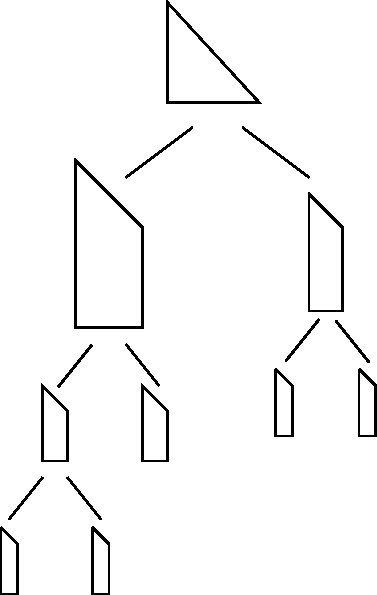
\includegraphics[width=0.9\textwidth]{figures/etree}}%
      \only<2>{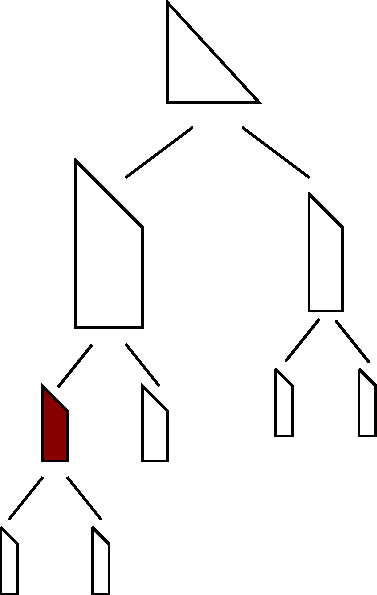
\includegraphics[width=0.9\textwidth]{figures/etree2}}%
      \only<3>{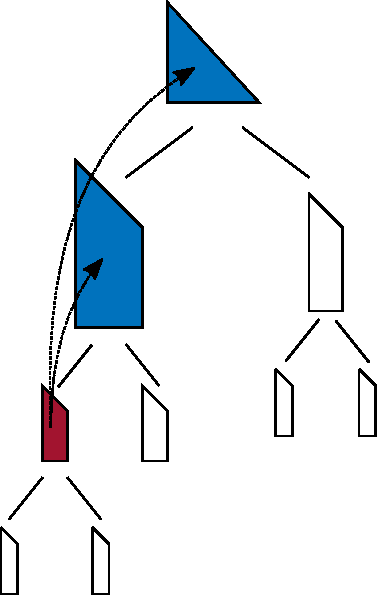
\includegraphics[width=0.9\textwidth]{figures/etree3}}%
    \end{column}

    \end{columns}

\end{frame}

\begin{frame}{The Sequential Task Flow Model}
  
  \alert{Sequential Task Flow} (STF) programming model:

  \begin{itemize}
  \item Tasks are submitted to the runtime system following the
    \db{sequential algorithm}.
  \item The runtime analyses manipulated data and infers task
    dependencies in order to ensure the \db{sequential consistency} of
    the parallel code.
  \item The DAG is executed via a \db{dynamic scheduling} of the
    (ready) tasks on the architectures.
  \item The runtime may be capable of automatically handling the data
    transfer across the architecture.
  \item \db{Superscalar analysis} in processors: dependency detection
    between instructions in order to issue them in parallel.
  \end{itemize}
  
\end{frame}

\begin{frame}{Experiments}
  \texttt{\scriptsize
    \begin{tabular}{rlrl}
        \hline
        \# & Matrix                         & Flops ($10^{9}$) & Application/description  \\
        \hline
        1  & Schmid/thermal2                & 18.6             & Unstructured thermal FEM \\
        2  & Rothberg/gearbox               & 22.8             & Aircraft flap actuator   \\
        3  & DNVS/m\_t1                     & 23.4             & Tubular joint            \\
        4  & DNVS/thread                    & 35.7             & Threaded connector       \\
        5  & DNVS/shipsec1                  & 40.5             & Ship section             \\
        6  & GHS\_psdef/crankseg\_2         & 48.8             & Linear static analysis   \\
        7  & AMD/G3\_circuit                & 67.3             & Circuit simulation       \\
        8  & Koutsovasilis/F1               & 228              & AUDI engine crankshaft   \\
        9  & Oberwolfach/boneS10            & 297              & Bone micro-FEM           \\
        10 & ND/nd12k                       & 514              & 3D mesh problem          \\
        11 & JGD Trefethen/Trefethen\_20000 & 669              & Integer matrix           \\
        12 & ND/nd24k                       & 2080             & 3D mesh problem          \\
        13 & Oberwolfach/bone010            & 3910             & Bone micro-FEM           \\
        14 & GHS\_psdef/audikw\_1           & 5840             & Automotive crankshaft    \\
        \hline
      \end{tabular}}

  \vspace{0.5cm}
  
  \begin{itemize}
  \item \db{Symmetric positive-definite} matrices
  \item \db{Metis} nested disection ordering
  \item \alert{Machine}: 2 $x$ 14 cores E5-2695 v3 (Haswell) @ 2.30GHz
  \end{itemize}

\end{frame}

\begin{frame}[fragile,t]{The STF Sparse Cholesky Factorization}
  \lstinputlisting{listings/spllt-stf.F90}
\end{frame}

\begin{frame}{The Parametrized Task Graph Model}
  
  \alert{Parametrized Task Graph} (PTG) programming model:

  \begin{itemize}
  \item Uses a \db{compact representation} of the DAG which is problem
    size independent.
  \item The dataflow between tasks is \db{explicitly} encoded
    (i.e. task dependencies are explicitly given).
  \item The runtime handles the communications implicitly using the
    dataflow representation.
  \item Under some hypothesis, the dataflow information can be
    \db{automatically} extracted from the sequential code using a dedicated
    compiler: \alert{not in our case} unfortunately.
  \end{itemize}

\end{frame}

\end{document}
